
%(BEGIN_QUESTION)
% Copyright 2005, Tony R. Kuphaldt, released under the Creative Commons Attribution License (v 1.0)
% This means you may do almost anything with this work of mine, so long as you give me proper credit

En student bygger følgende regulerte AC-DC-strømforsyningskrets, men er misfornøyd med ytelsen:

$$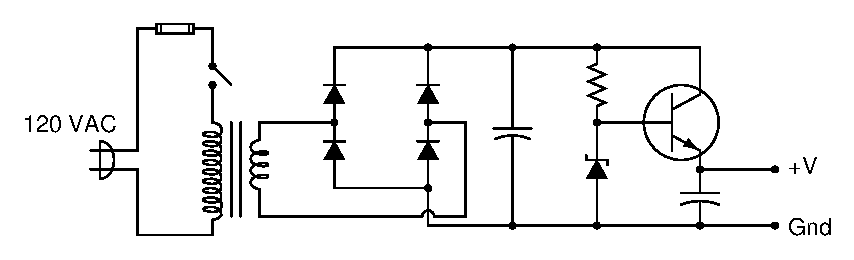
\includegraphics[width=15.5cm]{i01473x01.eps}$$

Spenningsreguleringen er ikke så god som studenten håpet. Ved belastning ``synker'' utgangsspenningen mer enn ønsket. Når zenerdiodens spenning måles under samme betingelser (ubelastet utgang kontra belastet utgang), ser man at også den synker noe. Studenten innser at en del av problemet er belastning av zenerdioden gjennom transistoren.

\vskip 10pt

For å forbedre spenningsreguleringen setter studenten inn en op-amp-koblet ``spenningsfølger'' mellom zenerdioden og transistoren:

$$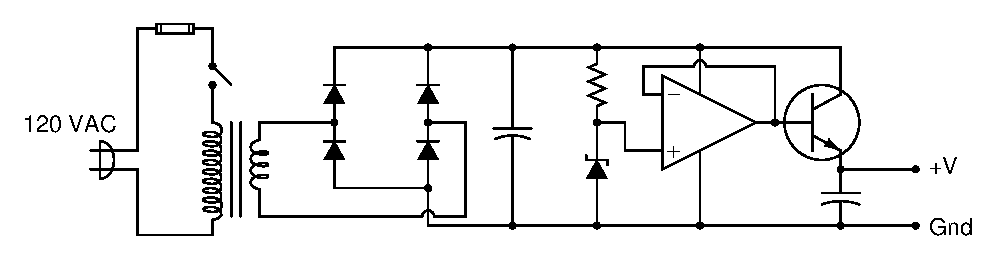
\includegraphics[width=15.5cm]{i01473x02.eps}$$

Nå er zenerdioden i praksis isolert fra transistorens belastningseffekter, og dermed også fra utgangsbelastningen. Op-ampen tar ganske enkelt zenerspenningen og gjenskaper den på transistorbasen, og leverer så mye strøm til transistoren som nødvendig uten å legge noen ekstra belastning på zenerdioden. Denne modifikasjonen forbedrer faktisk kretsens evne til å holde en stabil utgangsspenning ved varierende belastning, men det er fortsatt rom for forbedring.

\vskip 10pt

\filbreak

En annen student ser på den modifiserte kretsen og foreslår én liten endring som dramatisk forbedrer spenningsreguleringen:

$$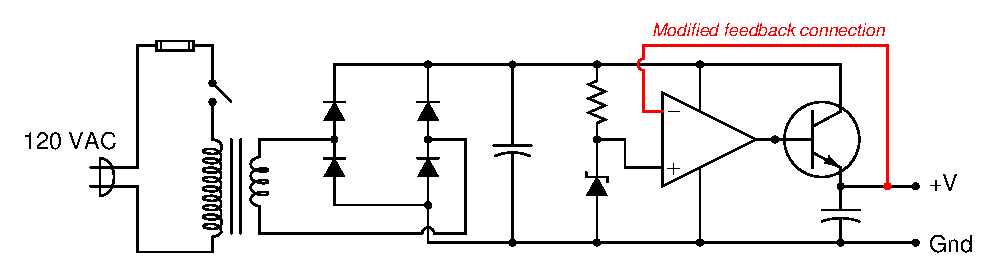
\includegraphics[width=15.5cm]{i01473x03.eps}$$

Nå holder utgangsspenningen seg stabil på zenerdiodens spenningsnivå, nesten uten ``sag'' under belastning. Den andre studenten er fornøyd med resultatet, men den første studenten forstår ikke hvorfor denne versjonen fungerer bedre enn den forrige. Hvordan ville du forklart den forbedrede ytelsen? Hvordan er forståelse av negativ tilbakekobling avgjørende for å kunne forstå kretsens virkemåte?

\vskip 10pt

Ett hint for å forklare op-ampens nye rolle er å relatere den til funksjonen til en {\it sløyferegulator}, der inngangssignalene representeres som {\it PV} og {\it SP}, og utgangssignalet som {\it Output}, mens transistoren fungerer som en {\it reguleringsventil}:

$$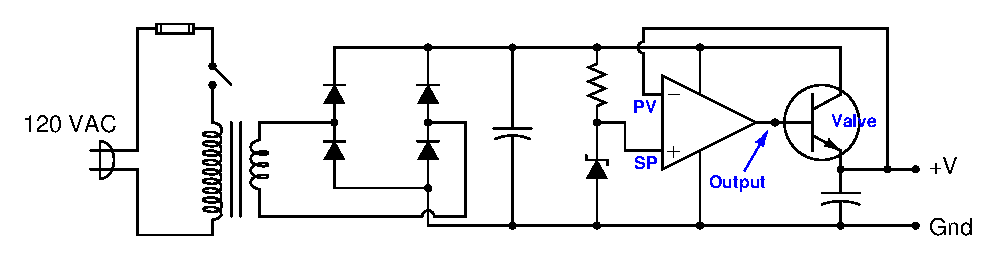
\includegraphics[width=15.5cm]{i01473x05.eps}$$

\vskip 20pt \vbox{\hrule \hbox{\strut \vrule{} {\bf Forslag til sokratisk diskusjon} \vrule} \hrule}

\begin{itemize}
\item{} Anta at zenerdiodens knekkspenning er 5.0 volt. Beregn utgangsspenningen for hver versjon av strømforsyningskretsen.
\item{} Jobber op-ampens ``sløyferegulator'' med {\it direktevirkning} eller {\it omvendtvirkning}?
\item{} Er gain i op-ampens ``sløyferegulator'' viktig for reguleringen av strømforsyningsspenningen? Med andre ord, blir spenningsreguleringen bedre eller dårligere hvis op-ampens interne (åpen sløyfe) spenningsforsterkning endres?
\item{} Hva vil skje med denne spenningsregulatorkretsen hvis motstanden i serie med zenerdioden feiler åpen?
\item{} Hva vil skje med denne spenningsregulatorkretsen hvis tilbakekoblingsledningen mellom op-ampens inverterende inngang og strømforsyningens utgangsterminal feiler åpen?
\item{} Hva vil skje med denne spenningsregulatorkretsen hvis transistoren feiler åpen mellom kollektor og emitter?
\end{itemize}

\underbar{file i01473}
%(END_QUESTION)





%(BEGIN_ANSWER)

Med tilbakekoblingen flyttet til ny plass ``ser'' op-ampen nå lastspenningen ved utgangsterminalene, og kan korrigere for {\it alle} spenningstap i effekttransistoren. Med den forrige tilbakekoblingen (fra op-ampens utgang) kunne op-ampen bare regulere spenningen på transistorbasen, ikke på selve lasten.

%(END_ANSWER)





%(BEGIN_NOTES)

Den siste versjonen av spenningsregulatorkretsen lar op-ampen måle den faktiske utgangsspenningen, ikke bare styresignalet til transistoren, og dermed korrigere for enhver endring i transistorens spenningsfall.

\vskip 10pt

Dette er en av mine favorittoppgaver når studentene begynner å lære hvordan negativ tilbakekobling virker. Det er en glimrende ``lakmustest'' på forståelsen av negativ tilbakekobling: studenter som forstår hvordan og hvorfor negativ tilbakekobling virker, vil umiddelbart forstå betydningen av den endrede tilbakekoblingskoblingen; de som ikke forstår negativ tilbakekobling, vil ikke skjønne hvorfor denne kretsen fungerer i det hele tatt. Bruk så mye tid som nødvendig på denne kretsen, fordi den er nøkkelen til å forstå svært mange op-amp-kretser.

$$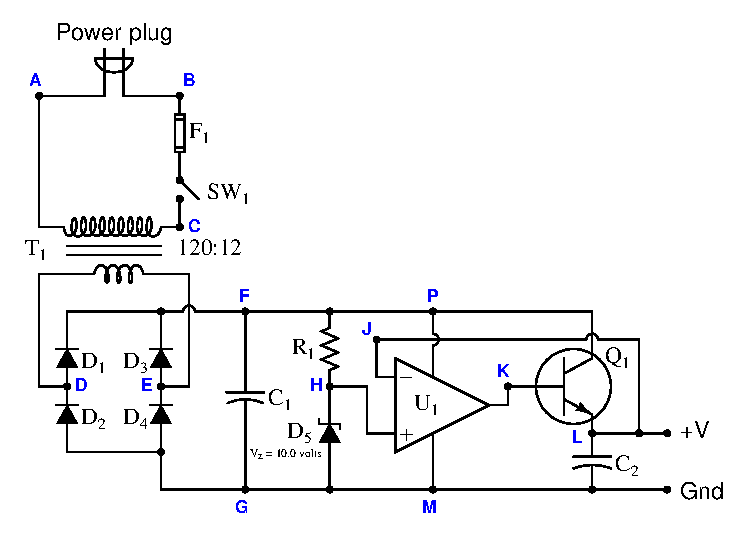
\includegraphics[width=15.5cm]{i01473x04.eps}$$

\vskip 20pt \vbox{\hrule \hbox{\strut \vrule{} {\bf Virtuell feilsøking} \vrule} \hrule}

Denne oppgaven egner seg godt som ``virtuell feilsøking''. Når du presenterer diagrammet for studentene, ser du først for deg en konkret feil i systemet. Deretter presenterer du ett eller flere symptomer på denne feilen (noe en operatør eller annen bruker kan observere). Studentene foreslår så ulike diagnostiske tester for å identifisere feiltype og feilplassering, som om de var teknikere som feilsøker systemet. Din oppgave er å fortelle hva resultatet av hver foreslåtte test ville blitt, og dokumentere resultatene slik at alle studentene kan se dem.

Under og etter øvelsen er det nyttig å stille oppfølgingsspørsmål som:

\begin{itemize}
\item{} Hva forteller resultatet av den siste diagnostiske testen om feilen?
\item{} Anta at resultatene fra den siste diagnostiske testen var annerledes. Hva ville det resultatet fortelle om feilen da?
\item{} Er den siste diagnostiske testen den beste vi kunne gjort?
\item{} Hva ville vært den ideelle rekkefølgen av tester for å diagnostisere problemet med færrest mulig trinn?
\end{itemize}

%INDEX% Electronics review: opamp used in a voltage regulator circuit

%(END_NOTES)

